%% LyX 2.4.4 created this file.  For more info, see https://www.lyx.org/.
%% Do not edit unless you really know what you are doing.
\documentclass[english,t]{beamer}
\usepackage{mathptmx}
\usepackage[T1]{fontenc}
\usepackage[latin9]{inputenc}
\usepackage{units}
\usepackage{amssymb}
\usepackage{cancel}

\makeatletter

%%%%%%%%%%%%%%%%%%%%%%%%%%%%%% LyX specific LaTeX commands.
%% Because html converters don't know tabularnewline
\providecommand{\tabularnewline}{\\}

%%%%%%%%%%%%%%%%%%%%%%%%%%%%%% Textclass specific LaTeX commands.
% this default might be overridden by plain title style
\newcommand\makebeamertitle{\frame{\maketitle}}%
% (ERT) argument for the TOC
\AtBeginDocument{%
  \let\origtableofcontents=\tableofcontents
  \def\tableofcontents{\@ifnextchar[{\origtableofcontents}{\gobbletableofcontents}}
  \def\gobbletableofcontents#1{\origtableofcontents}
}

%%%%%%%%%%%%%%%%%%%%%%%%%%%%%% User specified LaTeX commands.
\usetheme{Warsaw}
% or ...

\setbeamercovered{transparent}
% or whatever (possibly just delete it)
\setbeamercovered{invisible} %makes overlays invisible

%gets rid of navigation symbols
\setbeamertemplate{navigation symbols}{}

%\usepackage{hyperref}
%\usepackage[usenames,dvipsnames,table]{xcolor} %adds additional color options
\definecolor{links}{HTML}{2A1B81}
%\hypersetup{colorlinks,linkcolor=blue,urlcolor=links}

\usepackage{multicol}

\usepackage{hyperref}

\usepackage{tikz}
\usetikzlibrary{calc}
\usetikzlibrary{plotmarks}
\usetikzlibrary{shapes}
\usepackage{pgfplots} %\usepackage{pgfplots, pgfplotstable}
\pgfplotsset{compat=newest}
\usepackage{filecontents}  %allows in file data
\usepgfplotslibrary{statistics} %allows histogram stuff

\usepackage{forest} %%for tree diagram

\usepackage{calc}
\usepackage[nomessages]{fp}

\usepackage[super]{nth} %easy 1st, 2nd, etc

%\usepackage{advdate}    % Advancing/saving dates
\usepackage{datetime}   % Dates formatting
%\usepackage{datenumber} % Counters for dates

\usepackage[super]{nth}

\usepackage{etex}

\usepackage{fancybox}

%%table colors
%\usepackage[table]{xcolor}
\usepackage{colortbl}

\usepackage[outline]{contour}  %allows text halos

\usepackage{epsdice} %%dice font
\usepackage[misc]{ifsym}
\newfont\dice{dice3d} %%3d dice font

\contourlength{1pt} %sets halo width
%%example: \node at (0.75,0.5) {\contour{white}{\Large Text!}};
%%example:  \node [fill=white,inner sep=1pt] at (2.25,0.5) {\Large 			Text!};
%%example:  \node [fill=white,rounded corners=2pt,inner sep=1pt] at 			(3.75,0.5) {\Large Text!};

%%%%%%%%%%%%%%%%%%%%%%%%%%%
\def\formatdateny{\csname noyear\languagename\expandafter\endcsname\formatdate}
\def\noyearenglish#1, \the\@year{#1}
\let\noyearamerican\noyearenglish
\let\noyearbritish\noyearenglish

%%allows uncover with forest diagrams
\tikzset{
    invisible/.style={opacity=0,text opacity=0},
    visible on/.style={alt=#1{}{invisible}},
    alt/.code args={<#1>#2#3}{%
      \alt<#1>{\pgfkeysalso{#2}}{\pgfkeysalso{#3}} % \pgfkeysalso doesn't change the path
    },
}
\forestset{
  visible on/.style={
    for tree={
      /tikz/visible on={#1},
      edge={/tikz/visible on={#1}}}}}

%%%redefines column alignment to match vertically
%\define@key{beamerframe}{t}[true]{% top
  %\beamer@frametopskip=.2cm plus .5\paperheight\relax%
  %\beamer@framebottomskip=0pt plus 1fill\relax%
 % \beamer@frametopskipautobreak=\beamer@frametopskip\relax%
  %\beamer@framebottomskipautobreak=\beamer@framebottomskip\relax%
  %\def\beamer@initfirstlineunskip{}%
%}

%%provides pdf with 4 slides per page; don't forget to add 'handout' to remove overlays
%\usepackage{pgfpages}
%\pgfpagesuselayout{4 on 1}[a4paper, landscape, border shrink=7mm]
%\pgfpageslogicalpageoptions{1}{border code=\pgfusepath{stroke}}
%\pgfpageslogicalpageoptions{2}{border code=\pgfusepath{stroke}}
%\pgfpageslogicalpageoptions{3}{border code=\pgfusepath{stroke}}
%\pgfpageslogicalpageoptions{4}{border code=\pgfusepath{stroke}}
%%%Don't forget to add 'handout'

\makeatother

\usepackage{babel}
\begin{document}
%%data for exams%%
\begin{filecontents}{exam_data.csv} 
dist 
89
85 
33 
51 
74 
40 
92 
64 
68 
92 
84 
96 
98 
60 
85 
71 
96 
24 
87 
81 
64 
71 
58 
40
\end{filecontents}

\newcommand{\xmax}{2000}
\newcommand{\xmin}{0}
\newcommand{\xstep}{0} %must be xmin+n
\newcommand{\ymax}{500}
\newcommand{\ymin}{0}
\newcommand{\ystep}{0} %must be ymin+n

\newcounter{countEx} \setcounter{countEx}{0}
\newcounter{countProb} \setcounter{countProb}{0}
\resetcounteronoverlays{countEx} \resetcounteronoverlays{countProb}

\newcommand{\ex}[3]{
	\addtocounter{countEx}{1}
	\only<#1-#2>{\begin{exampleblock} {Example \chNum.\secNum.\arabic{countEx}.} #3	\end{exampleblock}}
}

\newcommand{\prob}[4]{
	\addtocounter{countProb}{1}
	\only<#1-#2>{\begin{exampleblock} {Problem  \chNum.\secNum.\arabic{countProb}.\,#3} #4	\end{exampleblock}}
}

\newcommand{\yline}[4]{
	(#2 - #4)/(#1 - #3)*(x - #1) + #2
}

\beamerdefaultoverlayspecification{<+->}

%%%%Chapter and Section numbers%%%%%
\newcommand{\chNum}{4}
\newcommand{\secNum}{1}
\newcommand{\secTitle}{Population, Sample, and Data}
\date{\formatdate{27}{10}{2014}}
\subtitle{Descriptive Statistics}

\makebeamertitle
\title[Section \chNum.\secNum: \secTitle]{Section \chNum.\secNum: \secTitle}

\subtitle{Finite Mathematics~~MTH 107~~Fall 2014}

\author{Dr.\,James Ashe}

\titlegraphic{\includegraphics[height=2.75cm]{/home/jim/JamesAshe/MHU/images/MarsHilUniversityLogo-Virtical.png}}

\institute{Mars Hill University}

\makebeamertitle 

%%True false command
\newcommand{\T}{\textcolor{green}{\contour{black}{T}}}
\newcommand{\F}{\textcolor{red}{\contour{black}{F}}}
\newcommand{\uT}[2]{\uncover<#1-#2>{\T}}
\newcommand{\uF}[2]{\uncover<#1-#2>{\F}}

%tkiz ball item 
\newcommand*\circled[1]{\tikz[baseline=(char.base)]
	{\node[circle,ball color=green!50!black!100, shade,   color=white,inner sep=1.2pt] (char) {\tiny #1};
	}
}
\begin{frame}{Statistics}

\begin{columns}


\column{5.5cm}

\vspace{4pt}
\begin{itemize}
\item []<2->\textbf{Descriptive Statistics:}

\begin{itemize}
\item <4->collecting,
\item <4->organizing,
\item <4->and summarizing data
\end{itemize}
\end{itemize}

\column{5.5cm}
\begin{itemize}
\item []<3->\textbf{Inferential Statistics}

\begin{itemize}
\item <5->drawing conclusions
\item <5->and
\item <5->making predictions
\end{itemize}
\end{itemize}
\end{columns}
\end{frame}

\begin{frame}{Population vs Sample}

\begin{example}
A CBS poll states that 44\% of NC voters will vote for Hagan, 41\%
for Tillis, and 2\% for Haugh.
\end{example}

\begin{columns}


\column{5.5cm}

\vspace{-15pt}
\begin{itemize}
\item []<2->\textbf{Descriptive Statistics:}
\item []<3->How was the data collected?
\item []<5->How can it be organized and displayed?
\end{itemize}

\column{5.5cm}

\vspace{-15pt}
\begin{itemize}
\item []<2->\textbf{Inferential Statistics}
\item []<6->How accurate is the poll?
\item []<6->How predicative is it?
\item []\uncover<4->{%%%%little circle in big%%%%%
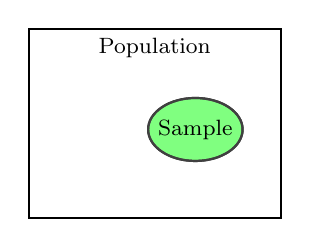
\begin{tikzpicture}[scale=.4]
	\def\circleA{(-25:2.25) ellipse (3.5 and 2.5)} %A
	\def\circleB{(0:1) circle (1)} %B
	\def\circleC{(-20:3.5) ellipse (1.5 and 1)} %C


	\colorlet{circle edgeA}{black!75} 
	\colorlet{circle areaA}{red!50}
	\colorlet{circle edgeB}{black!75} 
	\colorlet{circle areaB}{blue!50}
	\colorlet{circle edgeC}{black!75} 
	\colorlet{circle areaC}{green!50}

	\tikzset{
		filledA/.style={fill=circle areaA, draw=circle edgeA, thick},
		filledB/.style={fill=circle areaB, draw=circle edgeB, thick},
		filledC/.style={fill=circle areaC, draw=circle edgeC, thick},
		outlineA/.style={draw=circle edgeA, thick},
		outlineB/.style={draw=circle edgeB, thick},
		outlineC/.style={draw=circle edgeC, thick}
	}

	\begin{scope}[fill opacity=1.0]         
			%\fill[filledA] \circleA;
			%\fill[filledB] \circleB;
			\fill[filledC] \circleC;  
	\end{scope}
	
	\footnotesize
	\draw[outlineC] \circleC node {Sample} node[below = 5pt] {$$};
	\node[anchor=south] at (current bounding box.north) {}; 
	\draw[thick] (-2,-4) rectangle (6,2) node[anchor=north] at (current bounding box.north) {Population};
\end{tikzpicture} }
\end{itemize}
\end{columns}
\end{frame}

\begin{frame}{Population vs Sample}

\begin{columns}


\column{5.5cm}
\begin{block}<2->{Population}
 The set of all objects under study.
\end{block}

\begin{block}<3->{Sample}
 Any subset of the population.
\end{block}
\begin{itemize}
\item <5->We want a sample that is \emph{representative }of the population.
\item <6->Otherwise, any conclusions drawn will be useless. 
\end{itemize}

\column{5.5cm}
\begin{itemize}
\item []<2->Step 1 of any study is data collection.
\item []\uncover<4->{%%%%little circle in big%%%%%
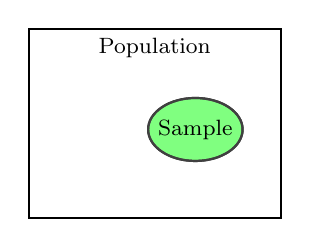
\begin{tikzpicture}[scale=.4]
	\def\circleA{(-25:2.25) ellipse (3.5 and 2.5)} %A
	\def\circleB{(0:1) circle (1)} %B
	\def\circleC{(-20:3.5) ellipse (1.5 and 1)} %C


	\colorlet{circle edgeA}{black!75} 
	\colorlet{circle areaA}{red!50}
	\colorlet{circle edgeB}{black!75} 
	\colorlet{circle areaB}{blue!50}
	\colorlet{circle edgeC}{black!75} 
	\colorlet{circle areaC}{green!50}

	\tikzset{
		filledA/.style={fill=circle areaA, draw=circle edgeA, thick},
		filledB/.style={fill=circle areaB, draw=circle edgeB, thick},
		filledC/.style={fill=circle areaC, draw=circle edgeC, thick},
		outlineA/.style={draw=circle edgeA, thick},
		outlineB/.style={draw=circle edgeB, thick},
		outlineC/.style={draw=circle edgeC, thick}
	}

	\begin{scope}[fill opacity=1.0]         
			%\fill[filledA] \circleA;
			%\fill[filledB] \circleB;
			\fill[filledC] \circleC;  
	\end{scope}
	
	\footnotesize
	\draw[outlineC] \circleC node {Sample} node[below = 5pt] {$$};
	\node[anchor=south] at (current bounding box.north) {}; 
	\draw[thick] (-2,-4) rectangle (6,2) node[anchor=north] at (current bounding box.north) {Population};
\end{tikzpicture} }
\item []<7->Step 2 is to organize it.
\end{itemize}
\end{columns}
\end{frame}

\begin{frame}{Data Organization}

\begin{columns}


\column{4.25cm}

\ex{1}{}{Number of children under five of each employee at a factory:

\hfill%
\begin{tabular}{ccccc}
0 & 2 & 1 & 0 & 3\tabularnewline
0 & 1 & 1 & 2 & 4\tabularnewline
1 & 0 & 1 & 1 & 0\tabularnewline
2 & 1 & 0 & 0 & 3\tabularnewline
3 & 0 & 0 & 1 & 2\tabularnewline
\end{tabular}\hfill}
\begin{itemize}
\item []
\item []
\end{itemize}

\column{6.5cm}
\begin{itemize}
\item []<2->Each element in this set is called a \textbf{data point}.
\item []<2->All the data is the \textbf{data set}. 
\item []<3->A table that lists each data point and its frequency is called
a \textbf{frequency distribution}.
\item []
\end{itemize}
\uncover<4->{%
\begin{tabular}{|c|c|c|}
\hline 
\rowcolor{yellow!50}\textbf{Num} & \textbf{Frequency} & \textbf{Relative Freq.}\tabularnewline
\hline 
\uncover<5->{0} & \uncover<6->{9} & \uncover<9->{$\nicefrac{9}{25}=36\%$}\tabularnewline
\hline 
\uncover<5->{1} & \uncover<7->{8} & \uncover<10->{$\nicefrac{8}{25}=32\%$}\tabularnewline
\hline 
\uncover<5->{2} & \uncover<7->{4} & \uncover<10->{$\nicefrac{4}{25}=16\%$}\tabularnewline
\hline 
\uncover<5->{3} & \uncover<7->{3} & \uncover<10->{$\nicefrac{3}{25}=12\%$}\tabularnewline
\hline 
\uncover<5->{4} & \uncover<7->{1} & \uncover<10->{$\nicefrac{1}{25}=4\%$}\tabularnewline
\hline 
\multicolumn{1}{c|}{} & \uncover<8->{$n=25$} & \uncover<11->{$\mbox{total}=100\%$}\tabularnewline
\cline{2-3}
\end{tabular}}
\end{columns}
\end{frame}

\begin{frame}{Grouped Data Organization}

\begin{columns}


\column{4.25cm}

\ex{1}{}{Grades from an exam are as follows:

\hfill%
\begin{tabular}{ccccc}
89 & 85 & 33 & 51 & 74\tabularnewline
40 & 92 & 64 & 68 & 92\tabularnewline
84 & 96 & 98 & 60 & 85\tabularnewline
71 & 96 & 24 & 87 & 81\tabularnewline
64 & 71 & 58 & 40 & \tabularnewline
\end{tabular}\hfill}
\begin{itemize}
\item <4->[]Max$=98$ and Min$=24$
\item <4->[]Range: $98-24-74$
\item <5->[]$74\div5=14.8\approx15$
\end{itemize}

\column{6.5cm}
\begin{itemize}
\item <2->Grouping data is necessary for more varied data sets;
\item <3->usually with 4 to 8 groups.
\end{itemize}
\only<4-11>{%
\begin{tabular}{|c|c|c|}
\hline 
\rowcolor{yellow!50}\textbf{Grade} & \textbf{Freq.} & \textbf{Relative Freq.}\tabularnewline
\hline 
\uncover<6->{$24\leq x<39$} & \uncover<8->{2} & \uncover<10->{$\nicefrac{2}{24}=8.3\%$}\tabularnewline
\hline 
\uncover<7->{$39\leq x<54$} & \uncover<8->{3} & \uncover<10->{$\nicefrac{3}{24}=12.5\%$}\tabularnewline
\hline 
\uncover<7->{$54\leq x<69$} & \uncover<8->{5} & \uncover<10->{$\nicefrac{5}{24}=20.8\%$}\tabularnewline
\hline 
\uncover<7->{$69\leq x<84$} & \uncover<8->{4} & \uncover<10->{$\nicefrac{4}{24}=16.7\%$}\tabularnewline
\hline 
\uncover<7->{$84\leq x<99$} & \uncover<8->{10} & \uncover<10->{$\nicefrac{10}{24}=41.7\%$}\tabularnewline
\hline 
\multicolumn{1}{c|}{} & \uncover<9->{$n=24$} & \uncover<11->{$\mbox{total}=100\%$}\tabularnewline
\cline{2-3}
\end{tabular}}\only<12-14>{%
\begin{tabular}{|c|c|c|}
\hline 
\rowcolor{yellow!50}\textbf{Grade} & \textbf{Freq.} & \textbf{Relative Freq.}\tabularnewline
\hline 
\uncover<12->{$24-38.9$} & \uncover<12->{2} & \uncover<12->{$\nicefrac{2}{24}=8.3\%$}\tabularnewline
\hline 
\uncover<13->{$39-53.9$} & \uncover<13->{3} & \uncover<13->{$\nicefrac{3}{24}=12.5\%$}\tabularnewline
\hline 
\uncover<13->{$54-68.9$} & \uncover<13->{5} & \uncover<13->{$\nicefrac{5}{24}=20.8\%$}\tabularnewline
\hline 
\uncover<13->{$69-83.9$} & \uncover<13->{4} & \uncover<13->{$\nicefrac{4}{24}=16.7\%$}\tabularnewline
\hline 
\uncover<13->{$84-98.9$} & \uncover<13->{10} & \uncover<13->{$\nicefrac{10}{24}=41.7\%$}\tabularnewline
\hline 
\multicolumn{1}{c|}{} & \uncover<14->{$n=24$} & \uncover<14->{$\mbox{total}=100\%$}\tabularnewline
\cline{2-3}
\end{tabular}}\only<15->{%
\begin{tabular}{|c|c|c|}
\hline 
\rowcolor{yellow!50}\textbf{Grade} & \textbf{Freq.} & \textbf{Relative Freq.}\tabularnewline
\hline 
\uncover<12->{$0-69.9$} & \uncover<12->{10} & \uncover<12->{$\nicefrac{10}{24}=41.7\%$}\tabularnewline
\hline 
\uncover<13->{$70-79.9$} & \uncover<13->{3} & \uncover<13->{$\nicefrac{3}{24}=12.5\%$}\tabularnewline
\hline 
\uncover<13->{$80-89.9$} & \uncover<13->{6} & \uncover<13->{$\nicefrac{6}{24}=25\%$}\tabularnewline
\hline 
\uncover<13->{$90-100$} & \uncover<13->{5} & \uncover<13->{$\nicefrac{5}{24}=20.8\%$}\tabularnewline
\hline 
\multicolumn{1}{c|}{} & \uncover<14->{$n=24$} & \uncover<14->{$\mbox{total}=100\%$}\tabularnewline
\cline{2-3}
\end{tabular}}
\end{columns}
\end{frame}

\begin{frame}{Histograms}

\begin{columns}


\column{6cm}

\only<2-2>{\begin{tikzpicture}[scale=.8]
\begin{axis}[     ybar,     ymin=0 ] 
\addplot +[hist={bins=5,data min=24,data max=98}] table [y index=0] {exam_data.csv}; 
\end{axis} 
\end{tikzpicture} }\only<3->{\begin{tikzpicture}[scale=.8]
\begin{axis}[     ybar,     ymin=0 ] 
\addplot +[hist={bins=10,data min=0,data max=100}] table [y index=0] {exam_data.csv}; 
\end{axis} 
\end{tikzpicture} }

\column{4.5cm}

\vspace{.5cm}

\only<1-2>{%
\begin{tabular}{|c|c|}
\hline 
\rowcolor{yellow!50}\textbf{Grade} & \textbf{Freq.}\tabularnewline
\hline 
$24-38.9$ & 2\tabularnewline
\hline 
$39-53.9$ & 3\tabularnewline
\hline 
$54-68.9$ & 5\tabularnewline
\hline 
$69-83.9$ & 4\tabularnewline
\hline 
$84-98.9$ & 10\tabularnewline
\hline 
\end{tabular}}\only<3->{%
\begin{tabular}{|c|c|c|}
\hline 
\rowcolor{yellow!50}\textbf{Grade} & \textbf{Freq.} & \textbf{Rel.}\tabularnewline
\hline 
$0-69.9$ & 10 & $41.7\%$\tabularnewline
\hline 
$70-79.9$ & 3 & $12.5\%$\tabularnewline
\hline 
$80-89.9$ & 6 & $25\%$\tabularnewline
\hline 
$90-100$ & 5 & $20.8\%$\tabularnewline
\hline 
\end{tabular}}
\end{columns}
\end{frame}

\begin{frame}{Histograms}

\ex{1}{}{200 randomly selected MHU graduates are listed below. Where
possible, deteremine what percent of the graduates had the following
ages:

}
\begin{columns}


\column{6cm}

\vspace{-.25cm}
\begin{itemize}
\item [a.]Less than 23

\begin{itemize}
\item <2->[]$\frac{1+4+52}{200}=0.285=28.5$
\end{itemize}
\item [b.]at most 20

\begin{itemize}
\item <3->[]$\frac{?}{200}$, not possible
\end{itemize}
\item [c.]at least 19 but less than 27

\begin{itemize}
\item <4->[]$\frac{52+48}{200}=0.5=50\%$
\end{itemize}
\end{itemize}

\column{4.5cm}

\vspace{-.25cm}

\begin{tabular}{|c|c|}
\hline 
\rowcolor{yellow!50}\textbf{Grade} & \textbf{Freq.}\tabularnewline
\hline 
$10\leq x<15$ & 1\tabularnewline
\hline 
$15\leq x<19$ & 4\tabularnewline
\hline 
$19\leq x<23$ & 52\tabularnewline
\hline 
$23\leq x<27$ & 48\tabularnewline
\hline 
$27\leq x<31$ & 31\tabularnewline
\hline 
$31\leq x<35$ & 16\tabularnewline
\hline 
$35\leq x<39$ & 29\tabularnewline
\hline 
$39$ and over & 19\tabularnewline
\hline 
\end{tabular}
\end{columns}
\end{frame}

\end{document}
